\subsection{Amplitudenmodulation (AM) S. 44}
Bei der Amplitudenmodulation formt das Nachrichtensignal die Amplitude des Trägersignals (carrier).

\vspace{.1cm}
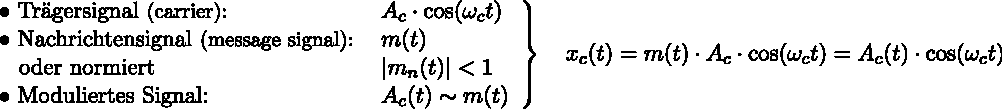
\includegraphics{content/06_amplitudenmodulation/AMbasic.pdf}

\vspace{.1cm}
$\rightarrow$ \textbf{Euler}:\hspace{.1cm} \efbox[linecolor=red]{$
		sin(t) = \frac{1}{2j}\cdot (e^{jt} - e^{.jt}) \;\;\;\;
		cos(t) = \frac{1}{2}\cdot (e^{jt} + e^{.jt})$}

\subsubsection{Frequenzmischer, Frequenzmultiplex S. 46}
Die Multiplikation des Signals $x(t)$ mit dem Träger $cos(\omega_0t)$ verschiebt das Spektrum nach $+/- \omega_0$.

\includegraphics{content/06_amplitudenmodulation/Frequenzmischer.pdf}

\newpage
\subsubsection{Gewöhnliche Amplitudenmodulation S. 44}
Bei der gewöhnlichen AM wird das Nachrichtensignal $m(t)$ mit einem DC offset angehoben um einen Nulldurchgang von $m(t)$ zu verhindern:\hspace{0.01cm} \vspace{.05cm} \efbox[linecolor=red]{$x_{AM}(t) = A_c \cdot (1+\mu \cdot m_n(t)) \cdot cos(\omega_c t)$ \;\; mit $|m(t)| \leq 1$ und Modulationsgrad $\mu$} \\
\textbf{Aufgrund des DC-Anteils ist die gewöhnliche AM nicht linear und nicht zeitinvariant!}

\paragraph{Modulation}
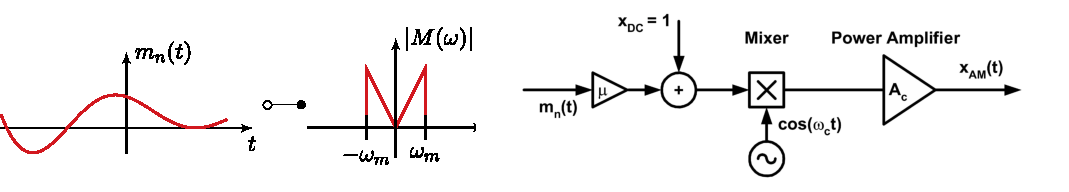
\includegraphics{content/06_amplitudenmodulation/AM_grafik.pdf}

\boxedeq{\begin{split}
		x_{_{AM}}(t) = (1 + \mu \cdot m_n(t)) \cdot A_C \cdot  \cos(\omega_c t)
		\; \;\;\; \laplace \;\;\; \; X_{AM}(\omega) = \frac{\mu A_c}{2}  (M(\omega - \omega_c) + 
		M(\omega + \omega_c)) \\ + \pi A_c [\delta (\omega - \omega_c) + 
		\delta (\omega + \omega_c)] \end{split}} \\

\begin{table}[H]
	\begin{tabularx}{\linewidth}{X X X}
		\begin{minipage}{\linewidth}
		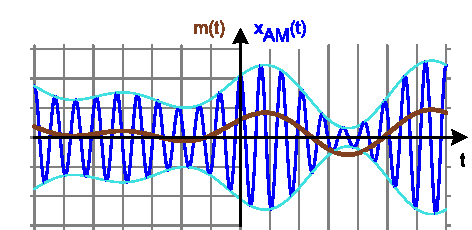
\includegraphics[width=\linewidth]{content/06_amplitudenmodulation/abbildung5_10.pdf}
		\end{minipage}
		&
		\begin{minipage}{\linewidth}
		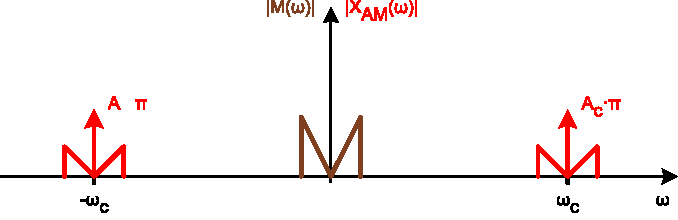
\includegraphics[width=\linewidth]{content/06_amplitudenmodulation/abbildung5_12.pdf}
		\end{minipage}
		&
		\begin{minipage}{1.05\linewidth}
			\textbf{DC-Anteil:} bewirkt, dass Carrier im Frequenzbereich nicht verschwindet \\
			\textbf{Modulationsindex $\mu$ :} $0 < \mu < 1$ \\
			$\mu > 1$ $\rightarrow$ Übermodulation \\
			 \efbox[linecolor=red]{$\mu = \frac{\max|x_{AM}|-min|x_{AM}|}{\max|x_{AM}|+min|x_{AM}|} $}
		\end{minipage}
	\end{tabularx}
\end{table}

\begin{tabular}{m{10cm} m{5cm}}
\paragraph{Demodulation}\mbox{ }
		\vspace{.2cm}
	
	\begin{list}{$\bullet$}{\setlength{\itemsep}{0cm} \setlength{\parsep}{0cm} 	\setlength{\topsep}{0cm}} 
		\item Hüllkurvendetektor (Envelope Detector) S.45
		\item Kohärente Produktdemodulation (siehe DSB-SC)
	\end{list}
\vspace{.5cm}
	\textbf{Bedingungen für Envelop-Demodulation}
	\vspace{.2cm}
	
	\begin{minipage}{\linewidth}
	\begin{list}{$\bullet$}{\setlength{\itemsep}{0cm} \setlength{\parsep}{0cm} 	\setlength{\topsep}{0cm}} 
		\item Umhüllende darf \textbf{nicht unter Null} fallen
		\item Modulationsindex $0 < \mu < 1$, bei Übermodulation fällt Umhüllende unter Null
		\item optimale Zeitkonstante des Hüllkurvendetektors \\
		$B_m < \frac{1}{RC} << f_c $ mit $B_m$: Bandbreite von $m(t)$
	\end{list}
	\end{minipage}
	
	&
	\begin{minipage}{0.4\linewidth}
		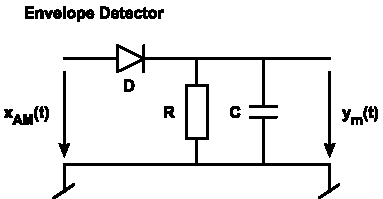
\includegraphics{content/06_amplitudenmodulation/abbildung5_9.pdf}
		
		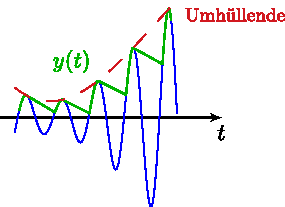
\includegraphics{content/06_amplitudenmodulation/envelope_graph.pdf}
	\end{minipage}

\end{tabular}

\newpage
\paragraph{Äquivalente Basisbanddarstellung der gewöhnlichen AM S. 47}
Vereinfacht gesagt wird die \textbf{Schwingung des Trägeres einfach weggelassen}, die Amplitude $A_c$ aber nicht.
\vspace{.3cm}

\begin{tabular}{m{.4\textwidth} m{.25\textwidth}}
	\begin{minipage}{\linewidth}
		Für Cosinusträger resultiert: \\
		\vspace{.5cm}
		\hspace{.3cm}\efbox[linecolor=red]{$x_{eq}(t) = A_c \cdot (1+ \mu m_n(t))$} \\
		In Abbildung rechts:
		$A_c = 1$, $\mu = \qty{25}{\%}$ (Länge des roten Strichs geht von 0.75 bis 1.25)
	\end{minipage}
	 & 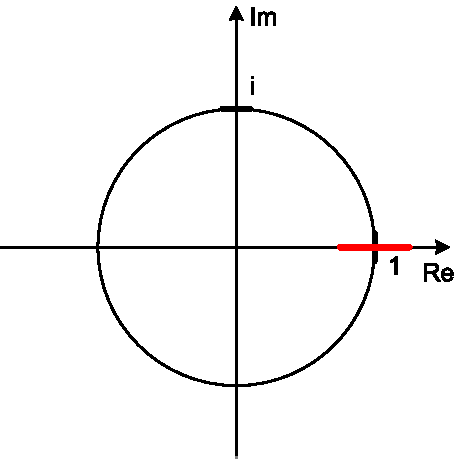
\includegraphics[width=.9\linewidth]{content/06_amplitudenmodulation/eqBaseCosine.pdf} \\ 
	 \begin{minipage}{\linewidth}
	 	Für Sinusträger muss wegen Euler noch ein $-j$ beibehalten werden! \\
	 	\vspace{.3cm}
	 	\hspace{.2cm}\efbox[linecolor=red]{$x_{eq}(t) = -j \cdot A_c \cdot (1+ \mu m_n(t))$}\\
	 	$A_c = 1$, $\mu = \qty{50}{\%}$ (Länge des roten Strichs geht von 0.50j bis 1.5j)
	 \end{minipage}
 & 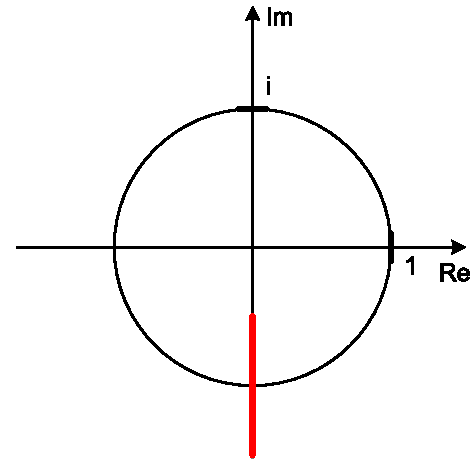
\includegraphics[width=.9\linewidth]{content/06_amplitudenmodulation/eqBaseSine.pdf}
\end{tabular}
\begin{minipage}{.3\textwidth}
	\begin{center}
		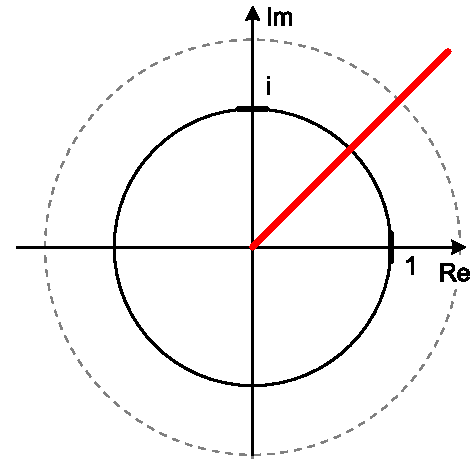
\includegraphics[width=.75\linewidth]{content/06_amplitudenmodulation/egBasePhaseShift.pdf}
	\end{center}
Cosinusträger mit Phasenverschobenem Trägersignal \\
\begin{center}
	\hspace{.1cm} \efbox[linecolor=red]{$x_{eq}(t) = \frac{1+j}{\sqrt{2}} \cdot A_c \cdot (1+\mu m_n(t))$}
\end{center}
$A_c=1$ \\
$\mu = \qty{100}{\%}$
\end{minipage}

\paragraph{Leistungseffizienz der gewöhnlichen AM S. 49}
Unter der Effizienz $\eta$ der gewöhnlichen AM versteht man das Verhältnis von Signalleistung $P_s$ der \textbf{beiden Seitenbänder} zur Gesamtleistung $P_t$ des AM-Signals.
\begin{equation*}
	P_c = \frac{A_c^2}{2} \;\; \text{und} \;\; P_t = \frac{A_c^2}{2} + \frac{A_c^2 \mu^2P_m}{2} \rightarrow \eta = \frac{P_s}{P_t} = \frac{P_t - P_c}{P_t} = \frac{\mu^2P_m}{1+\mu^2P_m} = \frac{(\frac{\mu}{C})^2}{1+(\frac{\mu}{C})^2} = \frac{\mu^2 \cdot m^2_{rms}}{1+\mu^2 \cdot m^2_{rms}}
\end{equation*}
Die maximal mögliche Effizienz ($\mu = \qty{100}{\%}$) beträgt \qty{33}{\%}. Bei $\mu = \qty{50}{\%}$ sind noch \qty{11.1}{\%} möglich.

\subsubsection{DSB-SC - Zweiseitenbandamplitudenmodulation ohne Träger S. 51}
Double-Sideband Suppressed-Carrier Modulation
\paragraph{Modulation}

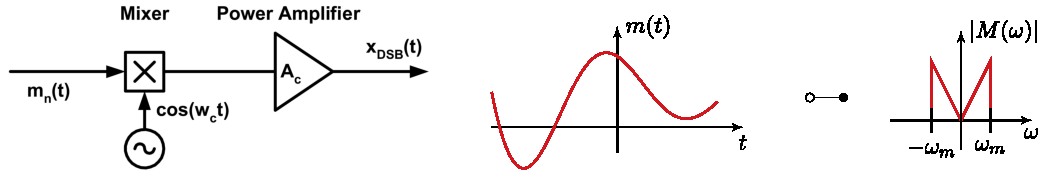
\includegraphics{content/06_amplitudenmodulation/DCBmodulation_grafik.pdf}
\begin{table}[H]
	\begin{tabularx}{\linewidth}{X X X}
		\begin{minipage}{\linewidth}
			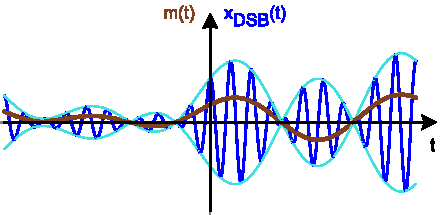
\includegraphics[width=\linewidth]{content/06_amplitudenmodulation/abbildung5_17.pdf}
		\end{minipage}
		&
		\begin{minipage}{\linewidth}
			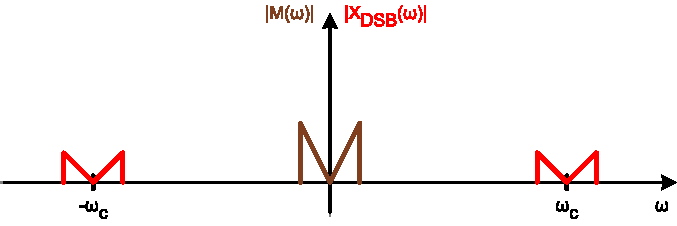
\includegraphics[width=\linewidth]{content/06_amplitudenmodulation/abbildung5_18.pdf}
		\end{minipage}
		&
		\begin{minipage}{1\linewidth}
			\textbf{Bandbreite:} \\$X(\omega) = 2 \cdot \text{ Bandbreite } M(\omega)$ \\
			\textbf{Amplitude:} \\$1/2 \text{ Amplitude } M(\omega)$\\
			(wenn $A_c = 1$)
		\end{minipage}
	\end{tabularx}
\end{table}
\textbf{DSB-SC ist linear, aber nicht zeitinvariant!} Trotzdem wird AM oft als lineare Modulation bezeichnet. Weil bei DSB-C und gewöhnlicher AM das Spektrum nur verschoben wird.

\paragraph{Demodulation S. 53}
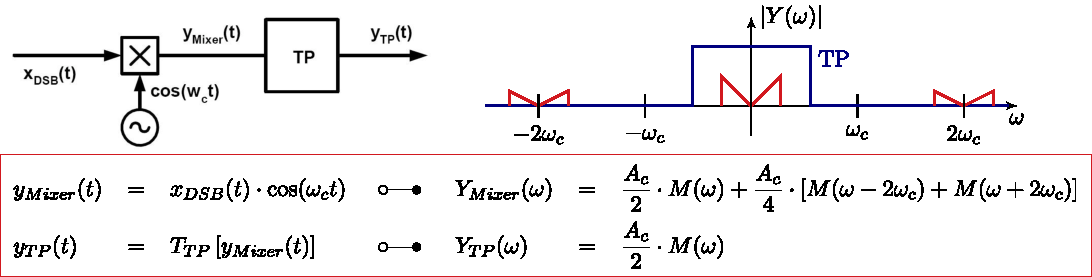
\includegraphics{content/06_amplitudenmodulation/DSB_SC_demodulation.pdf}

Das DSB-Signal wird mit einem sogenannten \textbf{synchronen Demodulator} oder \textbf{kohärenten Demodulator} zurückgewonnen. Weicht die \textbf{Frequenz oder die Phase} des demodulierten, lokalen Trägers von dem, des ursprünglichen Trägers ab, so ergibt sich eine \textbf{Abschwächung im demodulierten Signal}.

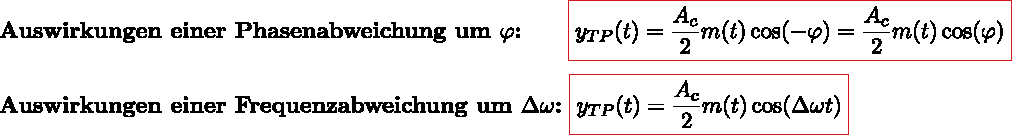
\includegraphics{content/06_amplitudenmodulation/demod_abweichung.pdf}

\subsubsection{Einseitenbandamplitudenmodulation (SSB) S. 53}
Bei der SSB Modulation wird \textbf{nur ein Seitenband übertragen}. Die Implementierung gegenüber gewöhnlicher AM und DSB ist komplexer.
\paragraph{Modulation - Filtermethode S. 54}
Mit einem Bandpassfilter kann entweder das USB (upper side band) oder das LSB (lower side band) unterdrückt werden um ein Einseitenband-Signal zu erhalten. Allerdings stellt dies \textbf{hohe Anforderungen an die Flankensteilheit} des Filters.

\paragraph{Modulation - Phasenmethode}
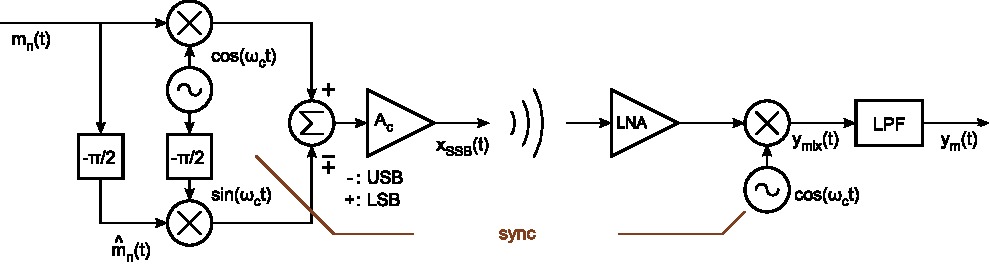
\includegraphics{content/06_amplitudenmodulation/abbildung5_23.pdf}
\begin{table}[H]
	\begin{tabularx}{\linewidth}{X X}
		\begin{minipage}{\linewidth}
			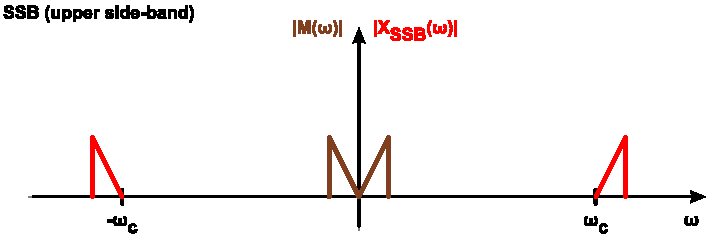
\includegraphics[width=\linewidth]{content/06_amplitudenmodulation/abbildung5_22_1.pdf}
		\end{minipage}
	&
	\begin{minipage}{\linewidth}
		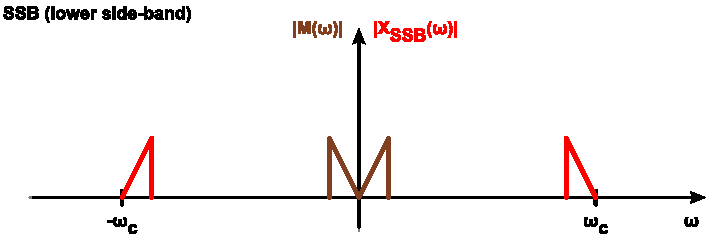
\includegraphics[width=\linewidth]{content/06_amplitudenmodulation/abbildung5_22_2.pdf}
	\end{minipage}
	\end{tabularx}
\end{table}
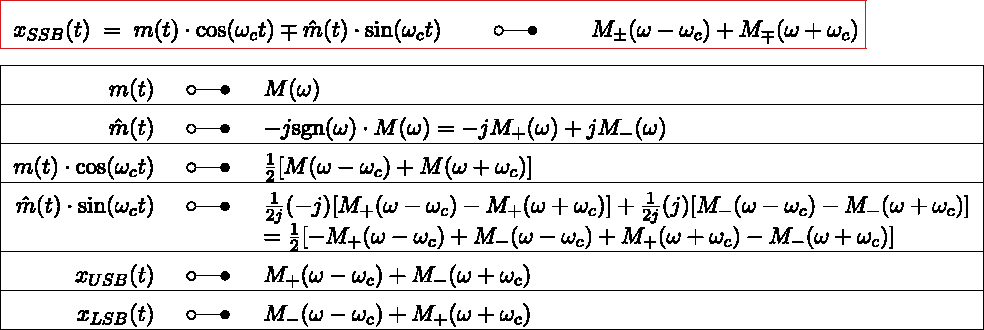
\includegraphics{content/06_amplitudenmodulation/SSB_phasenmethode.pdf}

\paragraph{Demodulation S. 56}
\textbf{Kohärente Demodulation ist erforderlich!}

\includegraphics{content/06_amplitudenmodulation/SSB_demod.pdf}

\subsubsection{Restseitenband-Amplitudenmodulation (VSB) S. 57}
Siehe auch Folie 23 NaT1\underline{ }3c; Restseitenband-AM ist ein Kompromiss zwischen:
\begin{list}{$\bullet$}{\setlength{\itemsep}{0cm} \setlength{\parsep}{0cm} 	\setlength{\topsep}{0cm}} 
	\item Bandbreiteneffizienz von SSB (1.25 x Bandbreite von SSB)
	\item Einfacher technischer Realisierung von DSB (keine extremen Anforderungen an Filtersteilheit)
\end{list}
\paragraph{Modulation}
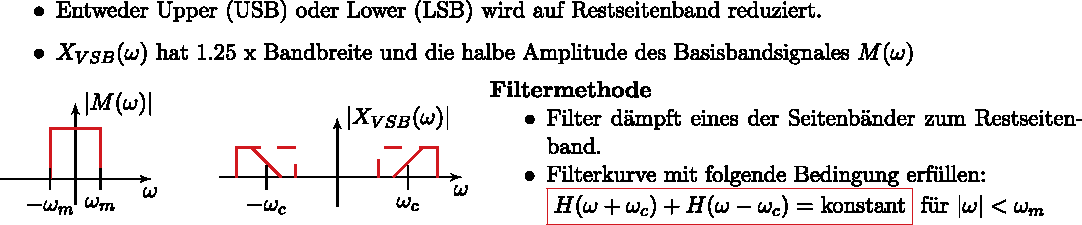
\includegraphics{content/06_amplitudenmodulation/VSB_mod.pdf}
\paragraph{Demodulation}
\textbf{Kohärente Demodulation ist erforderlich!}\\
Demodulation erfolgt gleich wie bei SSB-AM

\subsubsection{Quadraturamplitudenmodulation (QAM) S. 58}
Gleichzeitige Übertragung von zwei Basisbandsignalen im gleichen Frequenzband aber mit zwei orthogonalen Trägersignalen $cos(\omega_c t)$ und $sin(\omega_c t)$.\\
Vorteil: ebenso hohe Bandbreiteneffizienz wie SSB-AM \\
Nachteil: technisch aufwändiger als DSB-AM
\paragraph{Modulation und Demodulation S. 59}
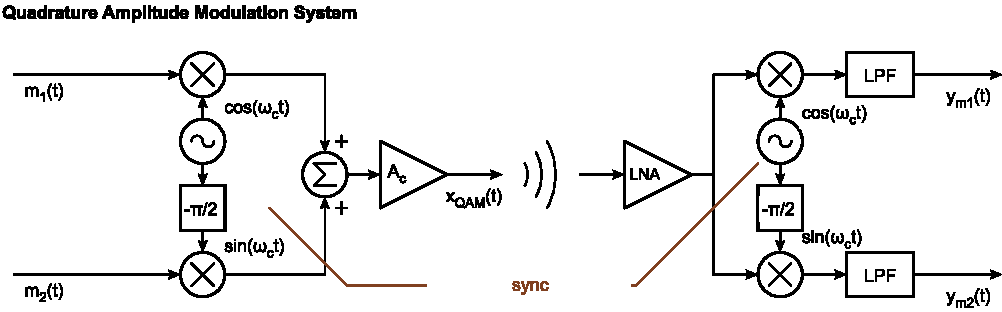
\includegraphics[width=.8\linewidth]{content/06_amplitudenmodulation/abbildung5_25.pdf}\\
\efbox[linecolor=red]{$B_{QAM} = 2\cdot max(B_{m1}, B_{m2}) $} $\rightarrow$ gleich wie DSB; Wenn $m_1$ die Hilberttrafo von $m_2$ ist, dann Bandbreite wie SSB $B_{SSB} = B_m$